\begin{frame}{Hardware - Raspberry Pi 2}
  \begin{center}
    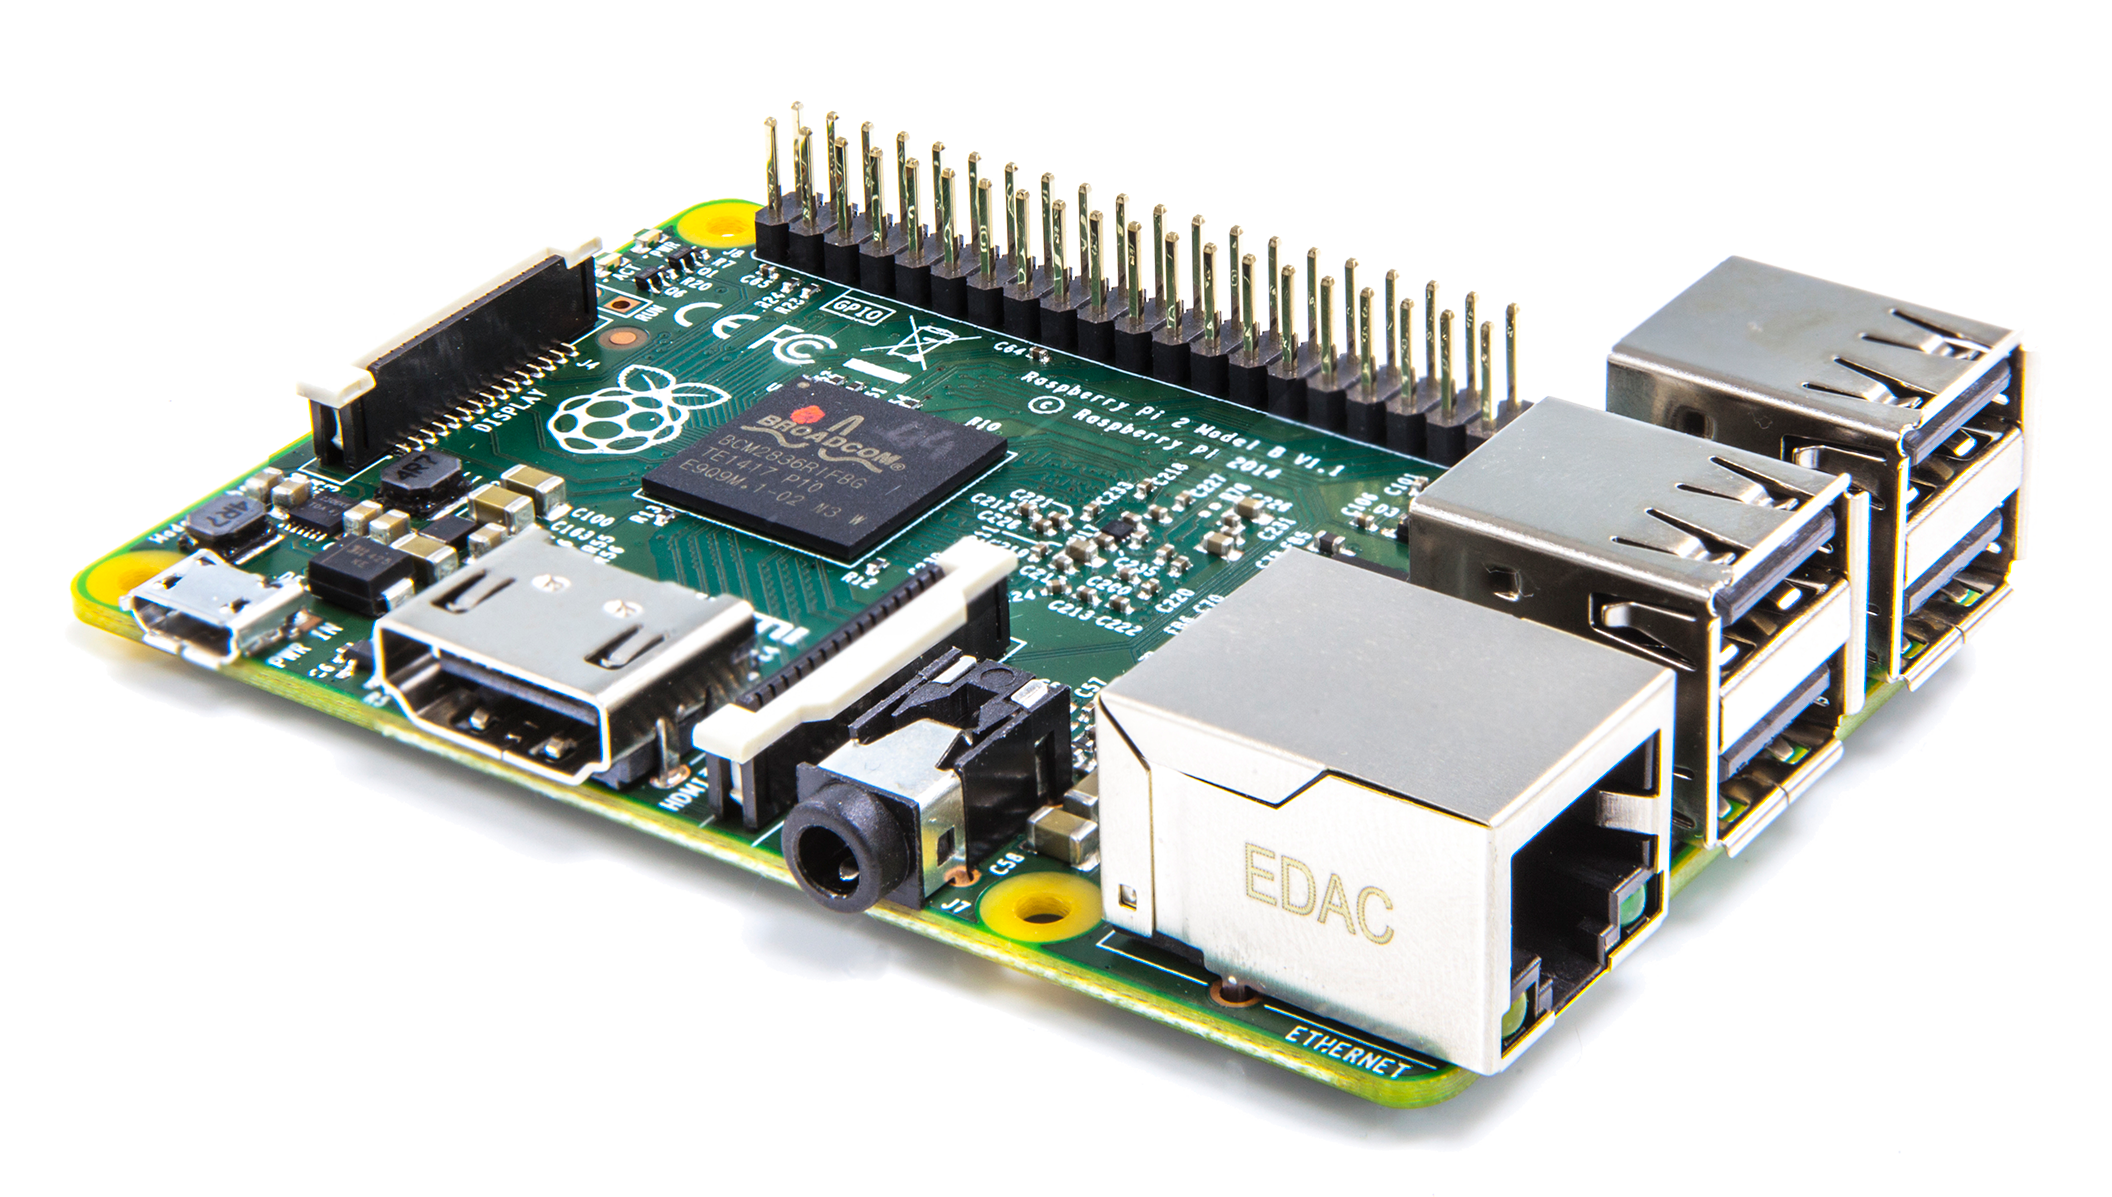
\includegraphics[width=\textwidth]{images/rpi2}
    \label{fig:rpi}
  \end{center}
\end{frame}

\begin{frame}{Hardware - Raspberry Pi 2 - Gründe}
  \Large
  \begin{itemize}
    \item Universell einsetzbar
    \item Sehr gutes Preis/Leistungs-Verhältnis
    \item Umfangreicher Support durch Community
    \item Große Basis unterstützter Software
    \item Einfach in der Handhabung
  \end{itemize}
\end{frame}

\begin{frame}{Hardware - Raspberry Pi 2 - Specs}
  \Large
  \center{
  \begin{tabular}{ l r }
%    L/B/H & \texttt{9,3 x 6,4 x 2,0 cm}\\
%    Gewicht & \texttt{45 g}\\
%    \\
    CPU & \texttt{ARM Cortex-A7}\\
    CPU-Kerne & \texttt{4}\\
    CPU-Takt & \texttt{900 MHz}\\
    RAM & \texttt{1 GB}\\
    \\
    Stromverbrauch & \texttt{max. 4 W} \\
    Preis & \texttt{\textasciitilde 40€}
  \end{tabular}}

\end{frame}

\begin{frame}{Hardware - RaspBee}
  \begin{center}
    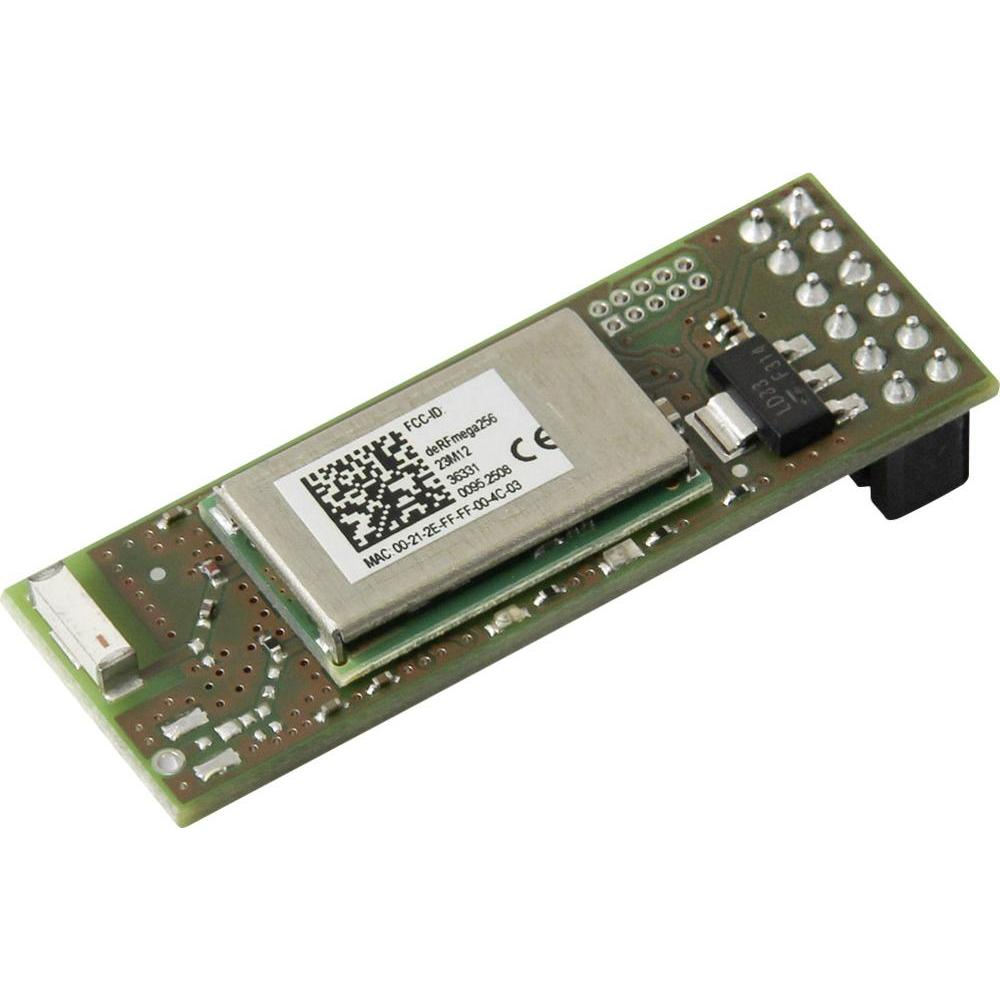
\includegraphics[width=\textwidth]{images/raspbee}
    \label{fig:rbee}
  \end{center}
\end{frame}

\begin{frame}{Hardware - RaspBee - Specs}
  \todo[inline]{Gimme those specs}
\end{frame}

\begin{frame}{Hardware}
  \begin{itemize}
	\item Philips Hue LED
  \end{itemize}
\end{frame}